%%%%%%%%%%%%%%%%%%%%%%%%%%%%%%%%%%%%%%%%%
% Beamer Presentation
% LaTeX Template
% Version 1.0 (10/11/12)
%
% This template has been downloaded from:
% http://www.LaTeXTemplates.com
%
% License:
% CC BY-NC-SA 3.0 (http://creativecommons.org/licenses/by-nc-sa/3.0/)
%
%%%%%%%%%%%%%%%%%%%%%%%%%%%%%%%%%%%%%%%%%

%----------------------------------------------------------------------------------------
%	PACKAGES AND THEMES
%----------------------------------------------------------------------------------------

\documentclass{beamer}

\mode<presentation> {

% The Beamer class comes with a number of default slide themes
% which change the colors and layouts of slides. Below this is a list
% of all the themes, uncomment each in turn to see what they look like.

%\usetheme{default}
%\usetheme{AnnArbor}
%\usetheme{Antibes}
%\usetheme{Bergen}
%\usetheme{Berkeley}
%\usetheme{Berlin}
%\usetheme{Boadilla}
%\usetheme{CambridgeUS}
%\usetheme{Copenhagen}
%\usetheme{Darmstadt}
%\usetheme{Dresden}
%\usetheme{Frankfurt}
%\usetheme{Goettingen}
%\usetheme{Hannover}
%\usetheme{Ilmenau}
%\usetheme{JuanLesPins}
%\usetheme{Luebeck}
\usetheme{Madrid}
%\usetheme{Malmoe}
%\usetheme{Marburg}
%\usetheme{Montpellier}
%\usetheme{PaloAlto}
%\usetheme{Pittsburgh}
%\usetheme{Rochester}
%\usetheme{Singapore}
%\usetheme{Szeged}
%\usetheme{Warsaw}

% As well as themes, the Beamer class has a number of color themes
% for any slide theme. Uncomment each of these in turn to see how it
% changes the colors of your current slide theme.

%\usecolortheme{albatross}
%\usecolortheme{beaver}
%\usecolortheme{beetle}
%\usecolortheme{crane}
%\usecolortheme{dolphin}
%\usecolortheme{dove}
%\usecolortheme{fly}
%\usecolortheme{lily}
%\usecolortheme{orchid}
%\usecolortheme{rose}
%\usecolortheme{seagull}
%\usecolortheme{seahorse}
%\usecolortheme{whale}
%\usecolortheme{wolverine}

%\setbeamertemplate{footline} % To remove the footer line in all slides uncomment this line
%\setbeamertemplate{footline}[page number] % To replace the footer line in all slides with a simple slide count uncomment this line

%\setbeamertemplate{navigation symbols}{} % To remove the navigation symbols from the bottom of all slides uncomment this line
}

\usepackage{graphicx} % Allows including images
\usepackage{booktabs} % Allows the use of \toprule, \midrule and \bottomrule in tables

%----------------------------------------------------------------------------------------
%	TITLE PAGE
%----------------------------------------------------------------------------------------

\title[Research Dissertation Process]{Research Dissertation Process } % The short title appears at the bottom of every slide, the full title is only on the title page

\author{Ferdinand Othieno} % Your name
\institute[SFAE] % Your institution as it will appear on the bottom of every slide, may be shorthand to save space
{
Strathmore University \\ % Your institution for the title page
\medskip
\textit{fothieno@strathmore.edu} % Your email address
}
\date{\today } % Date, can be changed to a custom date

\begin{document}

\begin{frame}
\titlepage % Print the title page as the first slide
\end{frame}

\begin{frame}
\frametitle{Outline} % Table of contents slide, comment this block out to remove it
\tableofcontents % Throughout your presentation, if you choose to use \section{} and \subsection{} commands, these will automatically be printed on this slide as an overview of your presentation
\end{frame}

%----------------------------------------------------------------------------------------
%	PRESENTATION SLIDES
%----------------------------------------------------------------------------------------

%------------------------------------------------
\section{Introduction} % Sections can be created in order to organize your presentation into discrete blocks, all sections and subsections are automatically printed in the table of contents as an overview of the talk
\subsection{The place of research at SFAE}
\subsection{Why research}
\section{Overview of the research process}
\subsection{The research process}
\section{SFAE 2015/16 Research project calendar}
\subsection{Student supervision}
\subsection{Research proposal}
\subsection{Research project report}
\subsection{Admin and support}
%------------------------------------------------
%------------------------------------------------
\begin{frame}
\begin{center}
\Huge Introduction
\end{center}
\end{frame}
%------------------------------------------------

\begin{frame}
\frametitle{\textbf{Why research}}
“Research is what I am doing when I do not know what I am doing.” - \textit{Wernher von Braun}\\~\\

"The outcome of any serious research can only be to make two questions grow where only one grew before." - \textit{Thorstein Veblen}\\~\\

No one undertakes research in Physics with the intention of winning a prize. It is the joy of discovering something no one knew before. - \textit{Stephen Hawking} 

\end{frame}

%------------------------------------------------

\begin{frame}
\frametitle{\textbf{Why research}}
\begin{block}{\textbf{Creation of knowledge}}
Basic research - Exploration to expand knowledge base.
\end{block}

\begin{block}{\textbf{Promote scholarship}}
(1) Engagement of students in the co-creation of knowledge.\\~\\
(2) Enhancement of teaching practice and insights 
\end{block}

\begin{block}{\textbf{Enhance decision making - Applied research}}
(1) Provide solutions for practitioners and technocrats.\\~\\
(2) Provide evidence for policy makers

\end{block}
\end{frame}

%------------------------------------------------

\begin{frame}
\frametitle{\textbf{Good research}}
\begin{block}{\textbf{Phenomena Versus Theory}}
Good applied research ideally does two things simultaneously.
\begin{enumerate}
\item It insightfully analyzes a phenomenon
\item It advances our theoretical understanding for how to deal with (an
aspect of) that phenomenon
\end{enumerate}

\end{block}
\end{frame}

%------------------------------------------------

\begin{frame}
\frametitle{\textbf{Good Applied Research}}
%\begin{figure}
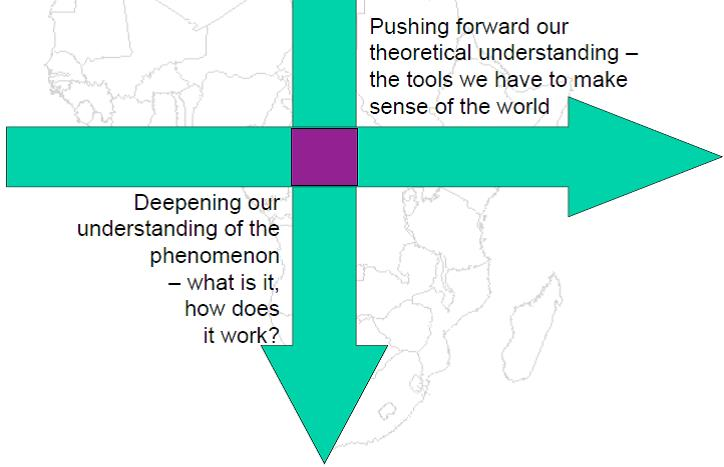
\includegraphics[width=\textwidth]{Applied_research}
%\end{figure}
\end{frame}

%------------------------------------------------
\begin{frame}
\begin{center}
\Huge The Research Process
\end{center}
\end{frame}
%------------------------------------------------%------------------------------------------------

\begin{frame}
\frametitle{\textbf{The research process}}
%\begin{figure}
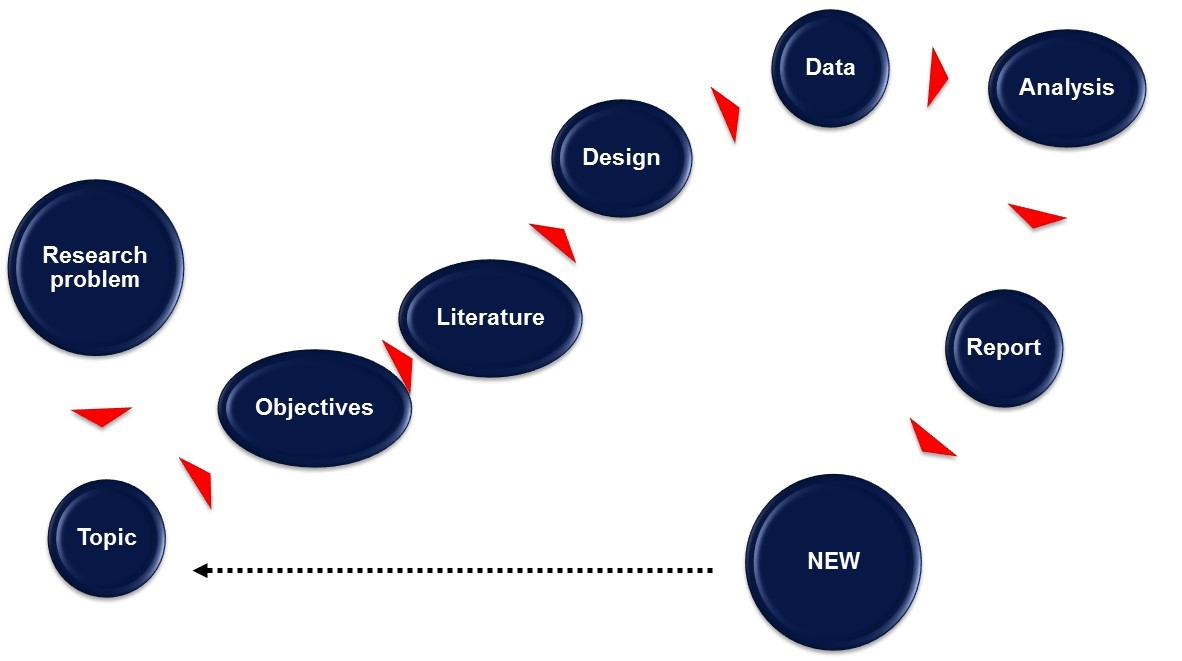
\includegraphics[width=\textwidth]{Research_proces}
%\end{figure}
\end{frame}


%------------------------------------------------

\begin{frame}
\Large{\centerline{SFAE 2015 Research Project Calendar}}
\end{frame}

%----------------------------------------------------------------------------------------
\begin{frame}
\frametitle{\textbf{SFAE 2015 Research Project Calendar}}
\begin{tabular} {|lr|}
\hline
\textbf{\large Activity} & \textbf{\large Timeline}\\~\\
\large Submission of Research Topic & \large 30 March 2015\\~\\
\large Confirmation of Assigned Supervisors & \large 22 April 2015\\~\\
\large Submission of Research Proposals & \large 3 July 2015\\~\\
\large Proposal Defenses & \large 27 - 31 July 2015\\~\\
\large Submission of Research Project & \large 2 November 2015\\~\\
\hline




\end{tabular}

\end{frame}
%------------------------------------------------

%------------------------------------------------

\begin{frame}
\Large{\centerline{Problem Statement}}
\end{frame}

%----------------------------------------------------------------------------------------

%------------------------------------------------

\begin{frame}
\frametitle{\textbf{Problem statement}}
\begin{block}{\textbf{A Research Problem is not the same as a business problem}}
Differentiate problem from symptom.
\begin{enumerate}
\item Insightfully analyze a phenomenon
\item Determine if problem or opportunity
\end{enumerate}
Differentiate business OR Market OR Policy problem from research problem. Always!
\begin{enumerate}
\item Business problems are sometimes symptoms of research problems 
\item Think of your Research Problem as the unknown part of the business problem.
\end{enumerate}
\end{block}
\end{frame}

%------------------------------------------------

\begin{frame}
\frametitle{\textbf{Problem statement - some reflections}}
\begin{enumerate}
\item A "Problem Statement" is a description of a difficulty or lack that needs to be solved or at least researched to see whether a solution can be found.\\
\item Can also be described as either a gap between the real and the desired or a contradiction between principle and practice.\\
\item Research Problem statements to have an outcomes based verb at or near the
beginning.\\
\begin{itemize}
\item Some good verbs - identify, formulate, construct, create etc\\
\item Bad verbs -understand, explore, investigate, discuss \\
\end{itemize}

\end{enumerate}

\end{frame}

%------------------------------------------------

%------------------------------------------------

\begin{frame}
\frametitle{\textbf{Problem statement - Qualities}}
\begin{enumerate}
\item Address a gap\\

\item Be significant enough to contribute to the existing body of research\\

\item Be one that will lead to more research \\

\item Render itself to be investigated via  collection of data \\

\item Be interesting to the researcher and suit his/her skills, time and resources\\
\item Should not have YES or NO answer\\
\item Should not suggest the solution OR finding that you expect,
otherwise you are introducing bias.\\
\item Be ethical\\

\end{enumerate}

\end{frame}

%------------------------------------------------

%------------------------------------------------

\begin{frame}
\frametitle{\textbf{Problem statement - Format}}
\begin{block}{\textbf{A persuasive problem statement has at least three parts}}
\begin{enumerate}
\item \textbf{The ideal:}  \large Describes a desired goal or ideal situation; explains how things should be\\

\item \textbf{The reality:}  \large Describes a condition that prevents the goal, state, or value in 1 from being achieved or realized at this time; explains how the current situation falls short of the goal or ideal.\\

\item  \textbf{The consequences:} \large Identifies the way you propose to improve the current situation and move it closer to the goal or ideal.\\


\end{enumerate}
\end{block}

\end{frame}

%------------------------------------------------

%------------------------------------------------

\begin{frame}
\frametitle{\textbf{Problem statement - Example}}
\begin{block}{\textbf{Persistent missing middle in Kenya - The ideal}}
\Large The government of Kenya has a goal to industrialize by the year 2030. In this regard it has encouraged growth oriented micro and small enterprises that should graduate into medium and large enterprises capable of contributing to the industrialization goal. There are several sessional papers (quote/cite) that contain specific measures to encourage and support MSEs.\\

\end{block}

\end{frame}

%------------------------------------------------

%------------------------------------------------

\begin{frame}
\frametitle{\textbf{Problem statement - Example}}
\begin{block}{\textbf{Persistent missing middle in Kenya - The reality}}
\Large Despite the said government efforts there is slow growth of micro into small enterprises  and even slower growth of small into medium scale enterprises(quote, show statistics). The government has officially acknowledged that there exists a "missing middle" in Kenya meaning that there is a gap between small and large enterprises in the country (cite, quote).\\

\end{block}

\end{frame}

%------------------------------------------------

\begin{frame}
\frametitle{\textbf{Problem statement - Example}}
\begin{block}{\textbf{Persistent missing middle in Kenya - The consequences}}
\Large Should the missing middle gap persist then the industrialization goal may be difficult to achieve. Need therefore arises to ascertain why despite government efforts there is a persistent missing middle\\

\end{block}

\end{frame}
%------------------------------------------------

\begin{frame}
\frametitle{\textbf{Problem statement - Exercise}}
\begin{block}{\textbf{What would be your corrected version?}}
\Large The large corporate companies need to be encouraged to assist small businesses in empowering them with the necessary skills and resources to grow. Corporate Social Responsibility is one avenue that small business can benefit from big business in this regard. My aim in this research is to establish if large companies are using corporate social responsibility to empower small business and, if not, how this can be done. Therefore the topic of this research is to identify the role of corporate social responsibility in empowering small business.\\

\end{block}

\end{frame}
%------------------------------------------------

\begin{frame}
\frametitle{\textbf{Problem statement - Exercise}}
\begin{block}{\textbf{Suggeste version}}
\Large The intention of this research is to establish the purposes for which large corporate are using their CSI / CSR programmes, with particular reference to whether and how they are using such programmes to empower small businesses, and, further, to gather ideas to expand such investments.\\

\end{block}

\end{frame}
%------------------------------------------------

\begin{frame}
\frametitle{\textbf{Problem statement - Counsel}}
\begin{block}{\textbf{No shortcuts}}
\Large Prepare to do a LOT of reading around your topic.
To be a “Master” of your topic, you need to know most of what has been
written about it, what the main ideas are, who the most important authors
are, and be able to differentiate credible sources from those that are not.\\

\end{block}

\end{frame}
%------------------------------------------------


\begin{frame}
\frametitle{\textbf{Any questions OR Clarification}}
%\begin{figure}

\includegraphics[width=\textwidth]{Questions}
%\end{figure}
\end{frame}


%------------------------------------------------

\begin{frame}
\frametitle{\textbf{Contact details}}
\begin{center}
Ferdinand Okoth Othieno\\
Director, Research\\ 
School of Finance and Applied Economics\\
Strathmore University\\
fothieno@Strathmore.edu\\

+254 721 722 872

\end{center}
\begin{block}{\textbf{Important Notice}}
\small The views and opinions expressed in this presentation are those of the presenter unless identified as those of other parties. The information contained herein is of a general nature and is intended for educational and instructional purposes only. Although the presenter has strived to provide accurate and timely information, there can be no guarantee that such information is accurate as of the date it is received or that it will continue to be accurate in the future. No one should act on such information without appropriate professional and scholarly advice after a thorough examination of the particular situation.

\end{block}
\end{frame}


%------------------------------------------------

\end{document}